\documentclass{../source/Experiment}

\major{信息工程}
\name{姚桂涛}
\title{A4 倒计时定时器设计、制作与调试}
\stuid{3190105597}
\college{信息与电子工程学院}
\date{\today}
\lab{东4-216}
\course{电子电路设计实验}
\instructor{李锡华、施红军、叶险峰}
\grades{}
\expname{倒计时定时器设计、制作与调试}
\exptype{研究实验}
\partner{郭含蕾}

\begin{document}
    \makecover
    \makeheader
    \section{实验目的}
        \begin{enumerate}
            \item 学习掌握用Arduino UNO 设计倒计时定时器
            \item 学习掌握PCB 电路板的设计和制作
            \item 学习掌握Arduino UNO 扩展板的设计与制作
            \item 学习掌握旋转编码器的使用
        \end{enumerate}
    \section{实验设计任务}
        \begin{enumerate}
            \item 用Arduino UNO 设计倒计时定时器,要求如下:设定倒计时时间若干(设定标准时间数组),通过旋转编码器选择,时间到时报警。
            \item 设计电路,完成相应器件的选择,制作Arduino UNO 扩展板。
            \item 编制与调试倒计时定时器程序。
            \item 将制作的扩展板与Arduino UNO 板组装后,进行系统联调。
        \end{enumerate}
    \section{主要仪器设备}
    Arduino UNO及其扩展版、旋转编码器、七段数码管、蜂鸣器、电阻若干、PNP三极管。
    \section{实验原理}
    本项目使用Arduino UNO 与其扩展板来实现倒计时定时器。下面对各部分模块进行说明。
        \subsection{旋转编码器}
        旋转编码器会游A、B两个输出,当不同方向转动旋转编码器的时候,可以通过A、B信号的不同变化进行区分。同时,旋转编码器还有一个开关输出。
        \subsection{7段数码管}
        7段数码管一般由8个发光二极管组成,其中由7个细长的发光二极管组成数字显示,另外一个圆形的发光二极管显示小数点。发光二极管的阳极连在一起的称为共阳极数码管,阴极连在一起的称为共阴极数码管。

        当发光二极管导通时,相应的一个点或一个笔画发光。控制相应的二极管导通,就能显示出各种字符。

        7段数码管有两种驱动显示方法,一个是静态显示驱动,一个是动态显示驱动。

        静态驱动也称直流驱动。静态驱动是指每个数码管的每一个段码都由一个单片机的I/O脚进行驱动,或者使用如BCD 码二-十进位计数器进行驱动。静态驱动的优点是编程简单,显示亮度高,缺点是占用I/O 脚多。

        动态驱动是将所有数码管的8 个显示笔划"a,b,c,d,e,f,g,dp "的同名端连在一起,另外为每个数码管的公共极COM 增加位元选通控制电路,位元选通由各自独立的I/O 线控制,当单片机输出字形码时,所有数码管都接收到相同的字形码,但究竟是那个数码管会显示出字形,取决于单片机对位元选通COM 端电路的控制,所以我们只要将需要显示的数码管的选通控制打开,该位元就显示出字形,没有选通的数码管就不会亮。

        透过分时轮流控制各个LED 数码管的COM 端,就使各个数码管轮流受控显示,这就是动态驱动。在轮流显示过程中,每位元数码管的点亮时间为1~2ms,由于人的视觉暂留现象及发光二极管的余辉效应,尽管实际上各位数码管并非同时点亮,但只要扫描的速度足够快,给人的印象就是一组稳定的显示资料,不会有闪烁感,动态显示的效果和静态显示是一样的,能够节省大量的I/O 埠,而且功耗更低。
        \subsection{时间报警电路}
        报警电路采用蜂鸣器。蜂鸣器按工作原理可分为压电式及电磁式的二大类:压电式蜂鸣器主要由多谐振荡器、压电蜂鸣片、阻抗匹配器及共鸣箱、外壳等组而发声;电磁式的蜂鸣器,则是用电磁的原理,通电时将金属振动膜吸下,不通电时依振动膜的弹力弹回。
        
    \section{实验设计}
        \subsection{总体设计}
        定时器总是处于两种状态之一:停止定时与定时运行。在停止定时状态,转动旋转编码器就可以改变定时时间;在定时运行状态,定时器倒计时,当倒计时结束后,蜂鸣器警报会响起。

        按下旋转编码器上的按钮可以对这两种状态进行切换。转动旋转编码器时定时时间并不是以秒为步进长度来改变时间,而是以一个标准时间数组来实现。

        同时通过EEPROM库用于保存最后使用的时间,所以每当这个装置上电时,它将记住最后一次使用的时间。
        \subsection{具体设计}
            \subsubsection{旋转编码器}
            旋转编码器1、3脚为信号A、B,2接地,4、5脚为开关信号。转动旋转编码器时,结合如下波形,通过A、B信号变化,可以判断是顺时针还是逆时针。
            \subsubsection{7段数码管}
            两个7段数码管的a~g引脚和dp引脚接Arduino板信号输出,同时A1(10)、A2(5)通过三极管连接到Arduino板,实现数码管的动态显示驱动。

            \subsubsection{蜂鸣器}
            报警模块我们选择了有源蜂鸣器。一个引脚接信号输出,另一个引脚接地。
    \section{实验过程}
            \subsection{电路图设计}
            根据参考资料,绘制出原理图。
            \begin{figure}[H]
                \centering
                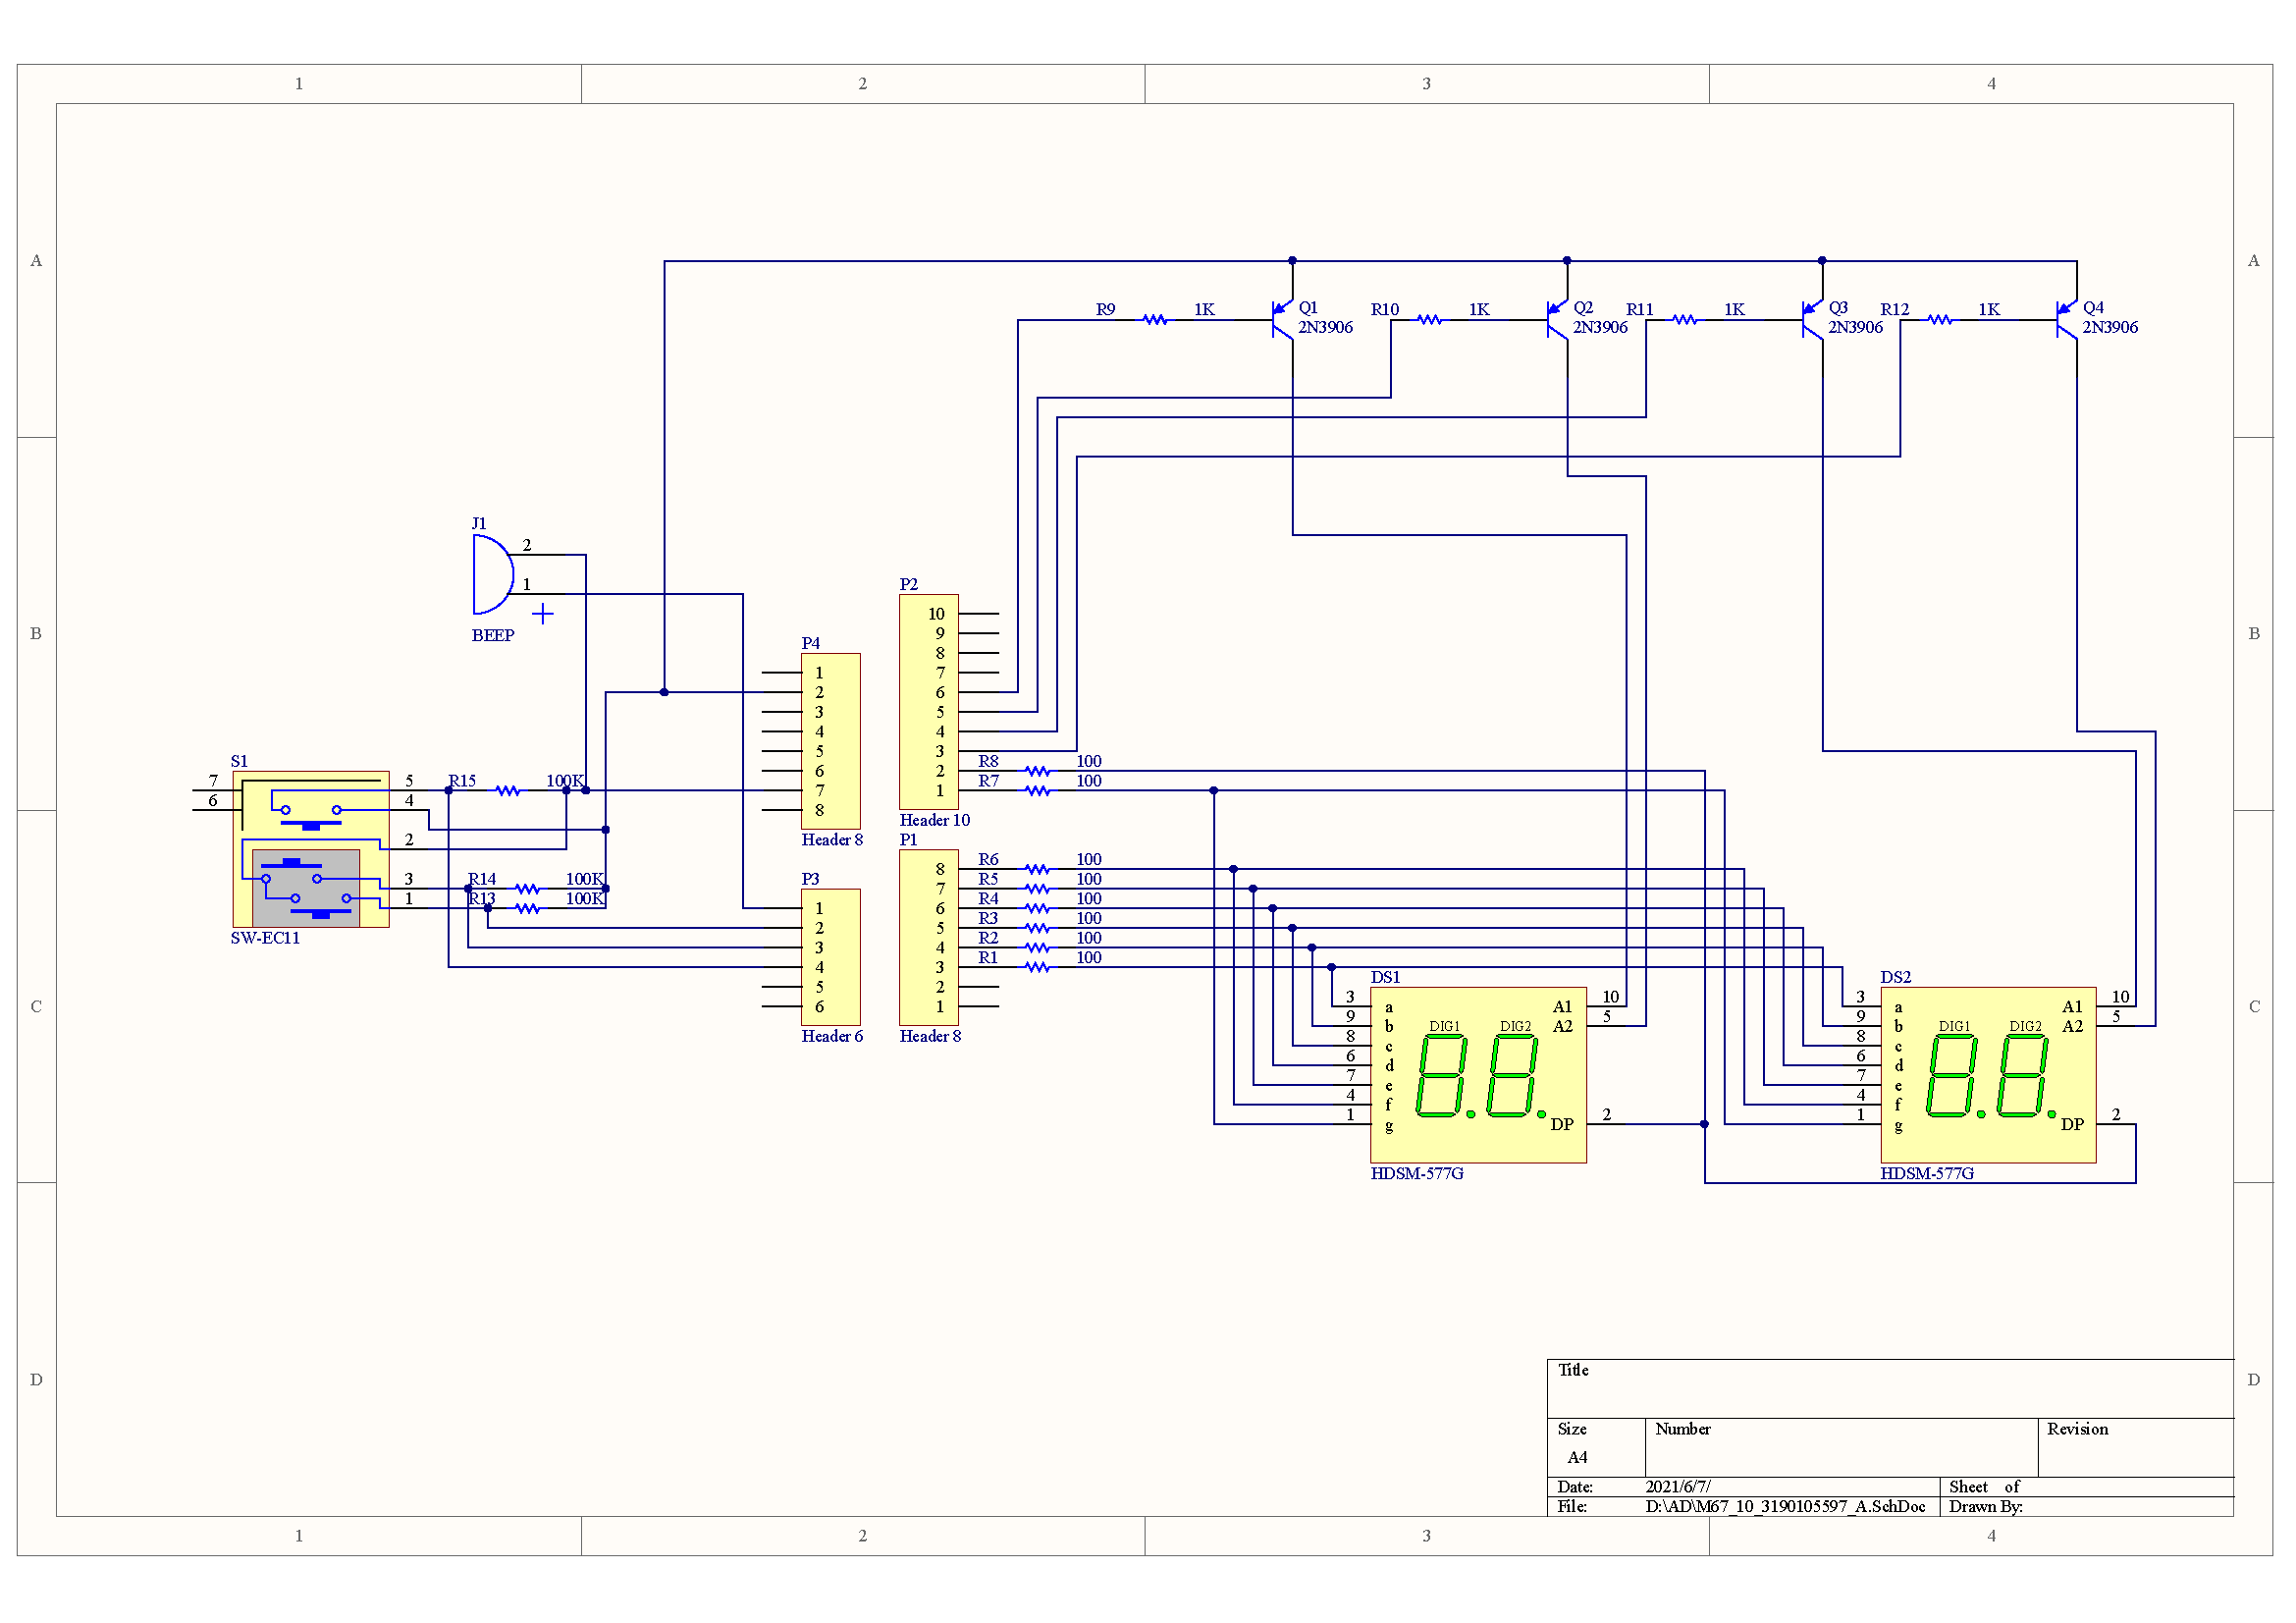
\includegraphics[width = 1\textwidth]{电路图}
                \caption{电路图}
            \end{figure}
            \subsection{面包板搭建}
            根据所绘制的电路图,我们在面包板上搭建出了具体的实物电路。
            \subsection{初步调试}
            排除电路搭建的问题后。从电路设计和代码两方面进行了调试。并完善了代码和原理图。
            
            部分关键代码:

            \begin{lstlisting}[name = 部分代码]
            //驱动数码管显示的引脚定义,0-13为数字引脚,14-19为模拟引脚
            int segmentPins[] = {2, 3, 4, 5, 6, 7, 8, 9};
            //用于驱动四个数码管,控制其开关数组最左对应最低位
            int displayPins[] = {10,11,12,13};
            // 时间序列
            int times[] = {5, 10, 15, 20, 30, 45, 100, 130,
            200, 230, 
            
            300, 400, 500, 600, 700, 800, 900, 1000, 1500, 2000,3000};
            int numTimes = 20;
            byte selectedTimeIndex;
            int timerMinute;
            int timerSecond;
            // 蜂鸣器开关
            int buzzerPin = A0;
            // 旋转编码器三个按钮
            int aPin = A1;
            int bPin = A2;
            int buttonPin = A3;

            boolean stopped = true; //初始为stopped
            byte digits[10][8] = {
                //a  b c d e f g.
                {1, 1, 1, 1, 1, 1, 0, 0}, //0
                {0, 1, 1, 0, 0, 0, 0, 0}, //1
                {1, 1, 0, 1, 1, 0, 1, 0}, //2
                {1, 1, 1, 1, 0, 0, 1, 0}, //3
                {0, 1, 1, 0, 0, 1, 1, 0}, //4
                {1, 0, 1, 1, 0, 1, 1, 0}, //5
                {1, 0, 1, 1, 1, 1, 1, 0}, //6
                {1, 1, 1, 0, 0, 0, 0, 0}, //7
                {1, 1, 1, 1, 1, 1, 1, 0}, //8
                {1, 1, 1, 1, 0, 1, 1, 0}  //9
            };

            \end{lstlisting}

            \begin{lstlisting}[name = 旋转编码器Arduino代码]
            int getEncoderTurn()
            {
                // return -1,0,or +1 
                static int oldA=LOW; 
                static int oldB=LOW; 
                int result = 0;
                int newA = digitalRead(aPin);
                //Serial.println(newA);
                int newB = digitalRead(bPin);
                Serial.println(newB);
                if (newA != oldA || newB != oldB)
                {
                    // something has changed
                    if(oldB == LOW && newB == HIGH){
                        result = -(oldA*2 - 1);
                    }
                }
                oldA = newA;
                oldB = newB;
                return result;
            }     
            \end{lstlisting}
            \subsection{PCB图绘制}
            确认所有元器件有对应的正确的封装后,进行了手动布线,绘制好PCB图。
            \begin{figure}[H]
                \centering
                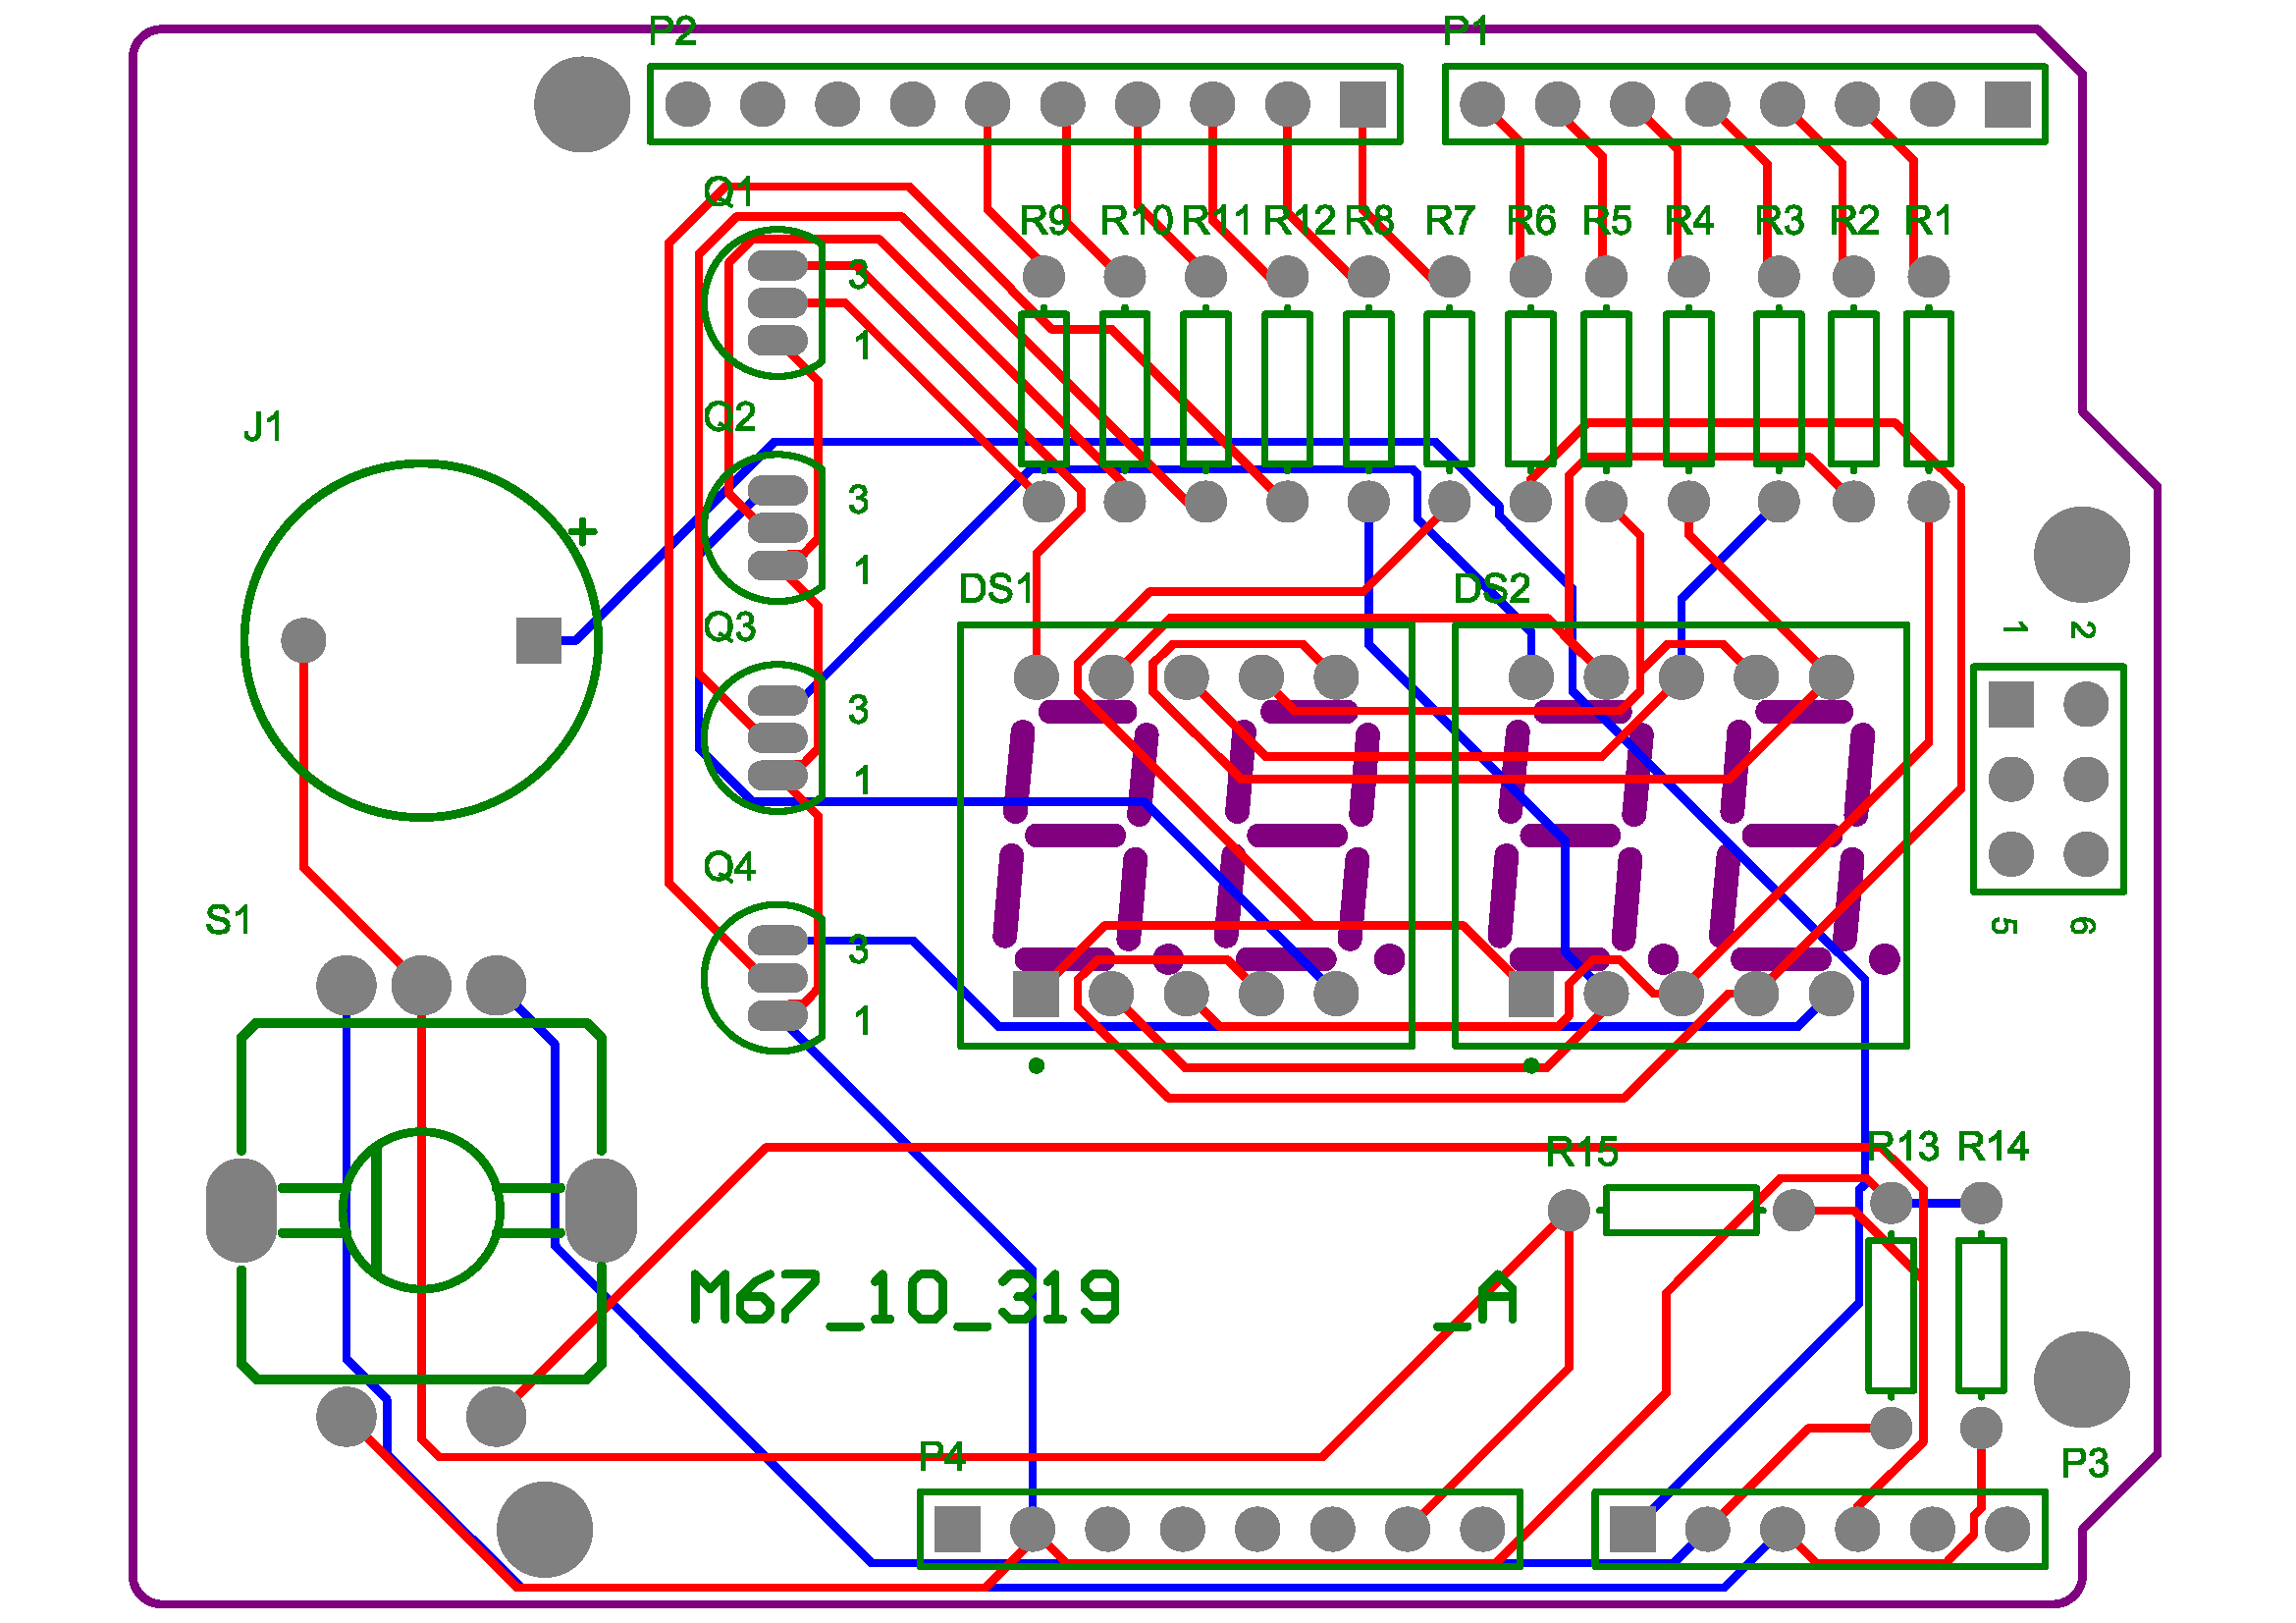
\includegraphics[width = 0.8\textwidth]{PCB}
                \caption{PCB图}
            \end{figure}
            \subsection{焊接}
            拿到PCB板后,按从低到高的原则进行元器件的焊接。
            \begin{figure}[H]
                \centering
                \includegraphics[width = 0.8\textwidth]{焊接}
                \caption{焊接图}
            \end{figure}
            \subsection{最终调试}
            最终调试,通过修改代码,解决了数码管刷新率太低而导致视觉效果差的问题。
            \begin{lstlisting}[name = 修改数码管刷新率]
            void process()
            {
                for (int i = 0; i < 50; i++) //修改此处i循环步数从而改变数码管刷新率
                {
                    int change = getEncoderTurn();
                    if (stopped)
                    {
                        changeSetTime(change);
                    }
                    else
                    {
                        updateCountingTime();
                    }
                }
                if (timerMinute == 0 && timerSecond == 0)
                {
                    digitalWrite(buzzerPin, HIGH);
                }        
            \end{lstlisting}

            \begin{figure}[H]
                \centering
                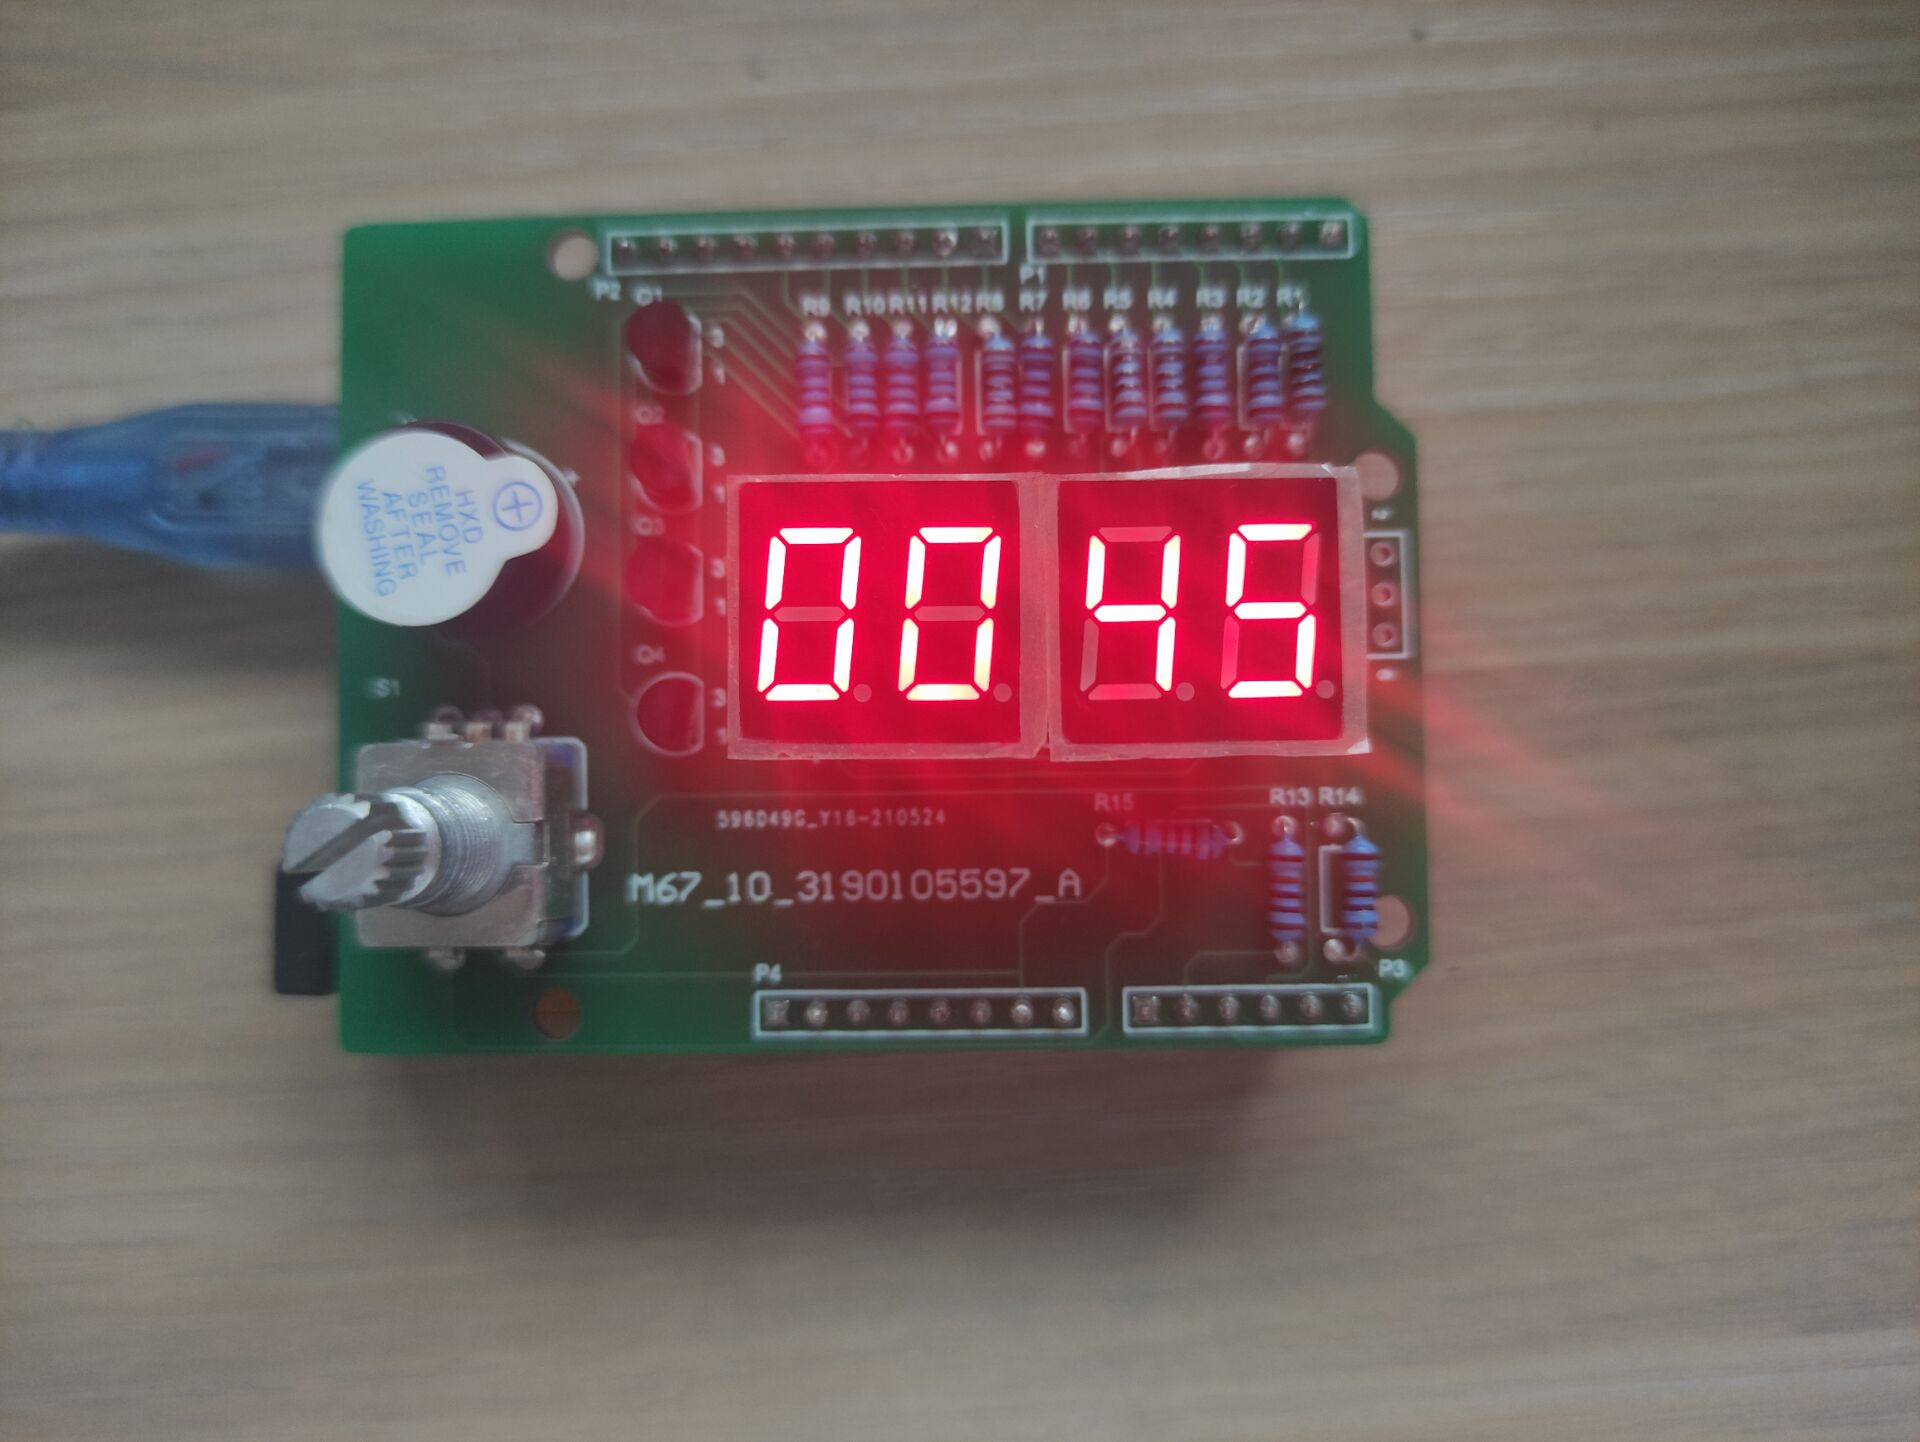
\includegraphics[width = 0.8\textwidth]{调试}
                \caption{最终成果图}
            \end{figure}
            
    \section{思考题}

    \subsection{将图4.15中的数码管换成共阴的,分别说明电路和程序要做怎样的修改。}

    电路:数码管的共阴极接地,a$\sim$dp管脚分别接一个pnp三极管的e极,三极管的c极接5V,b极接每个引脚的驱动信号。

    程序:数码管的驱动信号改为高电平点亮。
    \subsection{考虑倒计时定时器的应用,例如如何控制定时加热,简要介绍实现的电路。}

    增加元器件:继电器、加热器件

    电路设计:Arduino新增一个引脚(假设为18号引脚)控制继电器开关。继电器继而控制加热器件的加热与否。

    程序设计:当倒计时开始时,此时stop变量为0,通过stop变量作为判断,让18引脚输出高电平,控制继电器从而控制加热器件开始加热;倒计时结束时,stop为1,过stop变量作为判断,让18引脚输出低电平,控制继电器从而控制加热器件停止加热。
    \subsection{如何通过修改程序,消除秒钟滴答声。}
    修改代码中updateCountingTime模块如下:


    \begin{lstlisting}[name = 修改后的代码]
void updateCountingTime()
{
    static unsigned long lastMillis;
    unsigned long m = millis();

    if (m > (lastMillis + 1000) && (timerSecond > 0 || timerMinute > 0))
    {
        if (timerSecond == 0)
        {
            timerSecond = 59;
            timerMinute--;
        }
        else
        {
            timerSecond--;
        }
        lastMillis = m;
    }
}
    \end{lstlisting}
    \section{讨论与心得}
    刚开始实验的时候,我和搭档都不太清楚具体该做什么,于是我们开始研究来所给的参考文档。我们仔细阅读了文档,明白了所需要用到的数码管、旋转编码器等元器件的原理。并且阅读了参考代码,明白了该实验的程序原理。在这基础上,我们初步确定了我们的实验原理,并且在AD软件上搭建了初步的电路图。

    根据我们所搭建的电路图,我们在面包板上搭建出了具体的实物电路。

    但是当我们搭建好实物电路并开始调试时,发现电路无法正常地工作。首先最直接的问题就是数码管的显示错误,在检查数码管的电路连接没有问题后,我们便开始检查参考资料提供的代码是否有问题。在仔细检查后我们发现,代码中,显示数字6的字形代码有问题。解决了这个问题后,我们又发现数码管数字各个位显示的位置不对,在调整了代码中displayPins[ \, ] 部分的引脚后,解决了这一问题。最后数码管成功显示出了正确的数字。

    在之后的调试过程中,我们发现旋转编码器的功能错误,虽然电路能正常的显示数字,并且能进行倒计时,但是无法通过旋转编码器进行时间的设置。仔细分析了电路后,我们将电路错误原因定在了旋转编码器模块的搭建上。在仔细分析了附录有关旋转编码器的参考资料并且认真学习了旋转编码器的原理之后,我们发现了问题所在。为了解决这个问题,我们并没有按照附录的参考资料所给的电路图搭建旋转编码器,而是按自己的理解搭建其电路。并且在AD上修改了相应的电路图和代码中相应的部分。经过这一番调试后,电路成功运行。

    在电路能正常运行后,我们对照电路修订了电路图,便开始了PCB图的绘制。绘制PCB图时,我们发现有部分元器件并没有对应的PCB图,在查阅资料后发现是因为这些元器件没有对应的封装。在原理设计图更换了对应的封装后,解决了这一问题。

    一开始我们选择了自动布线,这样虽然非常的方便,但是仔细思考后发现这样并不能锻炼我们的能力 ,我们也无法从中学习到任何技能。于是我们转而选择了手动布线。最后设计出了较为满意的PCB图。

    拿到PCB板,我们便开始了焊接。在焊接到三极管的时候,由于三极管的三个引脚相邻很近,导致我多次将两个引脚焊接到一起。在多次尝试之后终于成功完成了焊接。

    最后测试时,只发现了一个小问题——数码管的刷新率太低,导致观感很差。在修改了代码后,这个问题得到了解决。

    经历这次实验,令我感悟最深的是要一步一个脚印,每一步做好之后,才去开始下一步。这样才能我们如果遇到问题,不会涉及到之前的过程,可以大大减少调试的难度和复杂度。比如这次实验,尤其是拿到PCB板之后,如果发现电路错误,是很难修改的,很有可能整个PCB板都需要重做。所以这就需要我们在印制PCB板之前确保我们的电路设计没有错误。我们小组在上交PCB设计图之前,仔仔细细检查了很多遍,在确认无误之后才上交。所以当我们拿到板完成焊接上电之后,并没有出现任何电路的问题。


\end{document}